
% here we go agane

\documentclass{article}

\usepackage[utf8]{inputenc}

\usepackage{amsmath, bm}
\usepackage{graphicx}
\usepackage{amssymb}
\usepackage{float}
\usepackage{caption}
\usepackage{subcaption}
\usepackage{hyperref}
\usepackage{tikz}
\usepackage{layout}
\usepackage{wrapfig}

\usepackage[margin=1in]{geometry}
\usepackage{listings}
\usepackage{xcolor}
\usepackage{color, colortbl}
\usepackage{textgreek}
\usepackage{mathrsfs}

\usepackage[moderate]{savetrees}

% 12 pt font
\renewcommand{\normalsize}{\fontsize{12pt}{\baselineskip}\selectfont}

\begin{document}

\title{4A7 Report \\ Climate Impact of Contrail Avoidance}
\author{5739G}
\date{December 2024}
\maketitle

\section{Introduction}
% evaluate the net climate impact of contrail avoidance

\section{Objectives}

\begin{itemize}
    \item Understand and quantify the climate impact of contrail avoidance using simple contrail and climate models.
    \item Investigate the impact of different aircraft fleets and fuels on the climate impact of contrail avoidance.
    \item Discuss limitations of simple models and compare to more complex models within the literature.
\end{itemize}

\subsection{Cases}

\begin{itemize}
    \item Baseline case, contrail avoidance with current aircraft fleet
    \item If the aircraft fleet is assumed to instead be fueled by liquified natural gas (LNG), which is taken to be methane
    \item If the gas turbines powering the fleet have a higher thermal efficiency (by an amount of your choosing) 
\end{itemize}

\section{Simplified Model}

The model consists of multiple coupled differential equations that are solved numerically.

\subsection{Radiative forcing from emissions}

The kerosene fuel burned by aircraft contains a mixture of alkanes of varying carbon chain lengths.
The combustion of each of these alkanes can be weighted by concentration to obtain an overall
emissions index of 3.15 in units mass of $CO_2$ per mass of kerosene fuel burned.
To get the total mass of fuel burn its required to know the flight paths and fuel burn rates for all aircraft.
This simply wasn't possible for all aircraft and times and so a months commercial flights dataset from EUROCONTROL [?] was used with a smaller list of aircraft fuel burn rates (kg/km) from wikipedia [?].
A correction factor was used to extrapolate the mass of fuel burned for unknown aircraft which was the ratio of total distance flown by all aircraft to aircraft of known fuel burn rate.
The CO2 emissions from flight was then estimated to be 0.31 Gt/Year.

The radiative forcing due to aircraft emissions of greenhouse gases can be estimated using the following simplified method.
In literature common units for carbon coming into or going out of the atmosphere is billions of tons of carbon per year ($\text{GtCyr}^{-1}$)
denoted $E(t)$, at the time $t$ in years. The carbon content of the atmosphere in units of billions of metric tons of carbon is denoted $C(t)$.
The current year is denoted $t=0$.
Measurements of E(t) and C(t) show that only roughly half of carbon emissions stay in the atmosphere, the rest is absorbed by the ocean and biosphere \cite{co2_modelling}.
This empirical observation is captured by the \emph{Constant Airborne Fraction Model}:

\begin{equation}
    \frac{dC}{dt} = k \left( E(t) - \frac{C(t)-C_\text{pre}}{\tau}\right)
\end{equation}

Where $k = 0.449$, $\tau = 276 $ years and $C_\text{pre} = 600$ GtC \cite{co2_modelling}.

Radiative forcing can be estimated using a relation by G. Myhre \cite{rf_greenhouse}.
This term adds a nonlinearity to the system of equations and is the reason for solving them numerically.

\begin{equation}
    \text{RF}_{\text{CO}_2} = 5.35 \ln \left( \frac{C}{C_0} \right)
\end{equation}

\subsection{Contrails}

The radiative forcing due to contrails is extrapolated from the work of D.S. Lee et al. \cite{contrail_radiative_forcing}.
An effective radiative forcing is taken as 57.4 mWm$^{-2}$.


\subsection{Temperature response}

These radiative forcing values provide an instantaneous metric for climate impact of emissions, however
the temperature response is a cumulative effect of radiative forcing over time.
This can simply be modelled by two heat reservoirs, one for shallow ocean and one for the deep ocean.
The temperature of the atmosphere $T_1$ and the temperature of the ocean $T_2$ are then given by the following equations.

\begin{align}
    C_1 \frac{dT_1}{dt} &= A_E[\text{RF} - \lambda(T - T_0) - k_m(T_1 - T_2)] \\
    C_2 \frac{dT_2}{dt} &= A_E[k_m(T_1 - T_2)]
\end{align}

Where $\lambda$ is the climate sensitivity parameter, $T_0$ is the pre-industrial temperature, $k_m$ is the heat exchange coefficient between the atmosphere and the ocean, and $C_1$ and $C_2$ are the heat capacities of the atmosphere and ocean respectively.
The values of these are set in table \ref{tab:temp_model_params}.

\begin{table}[H]
    \centering
    \begin{tabular}{ccc}
        \hline
        Parameter & Value & Unit \\
        \hline
        $T_0$ & 288 & $^\circ K$ \\
        $\lambda$ & 1.0 & $W/m^2K$ \\
        $k_m$ & 1.0 & $W/m^2K$ \\
        $C_1$ & $7.4\times 10^{22}$ & J/K \\
        $C_2$ & $5.3\times 10^{24}$ & J/K \\
        \hline
    \end{tabular}
    \caption{Temperature model parameters}
    \label{tab:temp_model_params}
\end{table}

AGWP can quantify cumulative radiative forcing.
AGTP can quantify the cumulative impact of increased temperatures such as changes in ecosystems and sea levels.
\begin{align}
    \text{AGWP} &= \int_0^T \text{RF}(t) dt \\
    \text{AGTP} &= \int_0^T \Delta T(t) dt
\end{align}

\subsection{Adaption for LNG fuel}

Liquid natural gas fuel will be taken as methane which has an emissions index lower than kerosine
of 2.75 kg $CO_2$ per kg methane burned.
This means a smaller emissions penalty of additional fuel consumption by avoiding contrails.

The Schmidt-Appleman criterion predicts contrails form if the mixture of exhaust gases and ambient air
transiently reaches or surpasses saturation with respect to liquid water.
It can be shown that the gradient of the mixing line is proportional to the $H_2O$ emissions index (ratio of mass $H_2O$ released per kg fuel burned) and inversely proportional to $LCV$ \ref{eq:SAC_gradient}.
Methane has a slightly higher calorific value $LCV$ ($50MJ/kg$) than kerosine ($43MJ/kg$) however the water vapour emissions index of methane (2.25) is significantly higher than kerosine (1.29).
By aligning this increased gradient to the saturation curve shows that contrails can form at higher temperatures.
Hence, more contrails form and cause a larger net radiative forcing making their avoidance more important.

However, to estimate the increased radiative forcing, the previous value by D.S. Lee et al. was multiplied by the ratio
of mixing line gradients.

\begin{equation}
    G = \frac{P EI_{H_2O} c_p}{\epsilon LCV (1-\eta)} \label{eq:SAC_gradient}
\end{equation}

Where P is static pressure, $c_p$ is specific heat capacity, $\epsilon = M_{H_2O}/M_{air} = 0.622$, $LCV$ is lower calorific value, and $\eta$ is thermal efficiency.

\subsection{Adaption for higher thermal efficiency}

A higher thermal efficiency reduces amount of fuel required for a flight, reducing the emissions.
However, it also reduces the term $(1-\eta)$ which G is inversely proportional and so the SAC mixing curve gradient increases.
Again this means that more contrails form and so avoidance may be more worthwhile for aircraft of higher thermal efficiency.

To estimate the increased radiative forcing the same technique as before where the value by D.S. Lee et al. was multiplied by the ratio
of mixing line gradients.


\subsection{Assumptions and Limitations}

Many assumptions and simplifications were made to perform the above analysis.
The validity of these are discussed with reference to more advanced models.

\subsubsection{Models}

The 
A number of assumptions were made in the calculation of fuel burn
Liquid natural gas only assumed to be methane

\subsubsection{Values}

% a list of all referenced models used in the report
% full description of model assumptions, limitations, and validation

% model of impact of contrails on climate

% require: fuel penalty associated with avoidance
%    meteorological conditions, aircraft type, altitude, and time of day
%    optimal routing and control strategies


% for additional cases may require different fuel consumption models
% but also the climate impact of sourcing methane from natural gas

\section{Results}
% tables and figures of results

\begin{figure}[H]
    \centering
    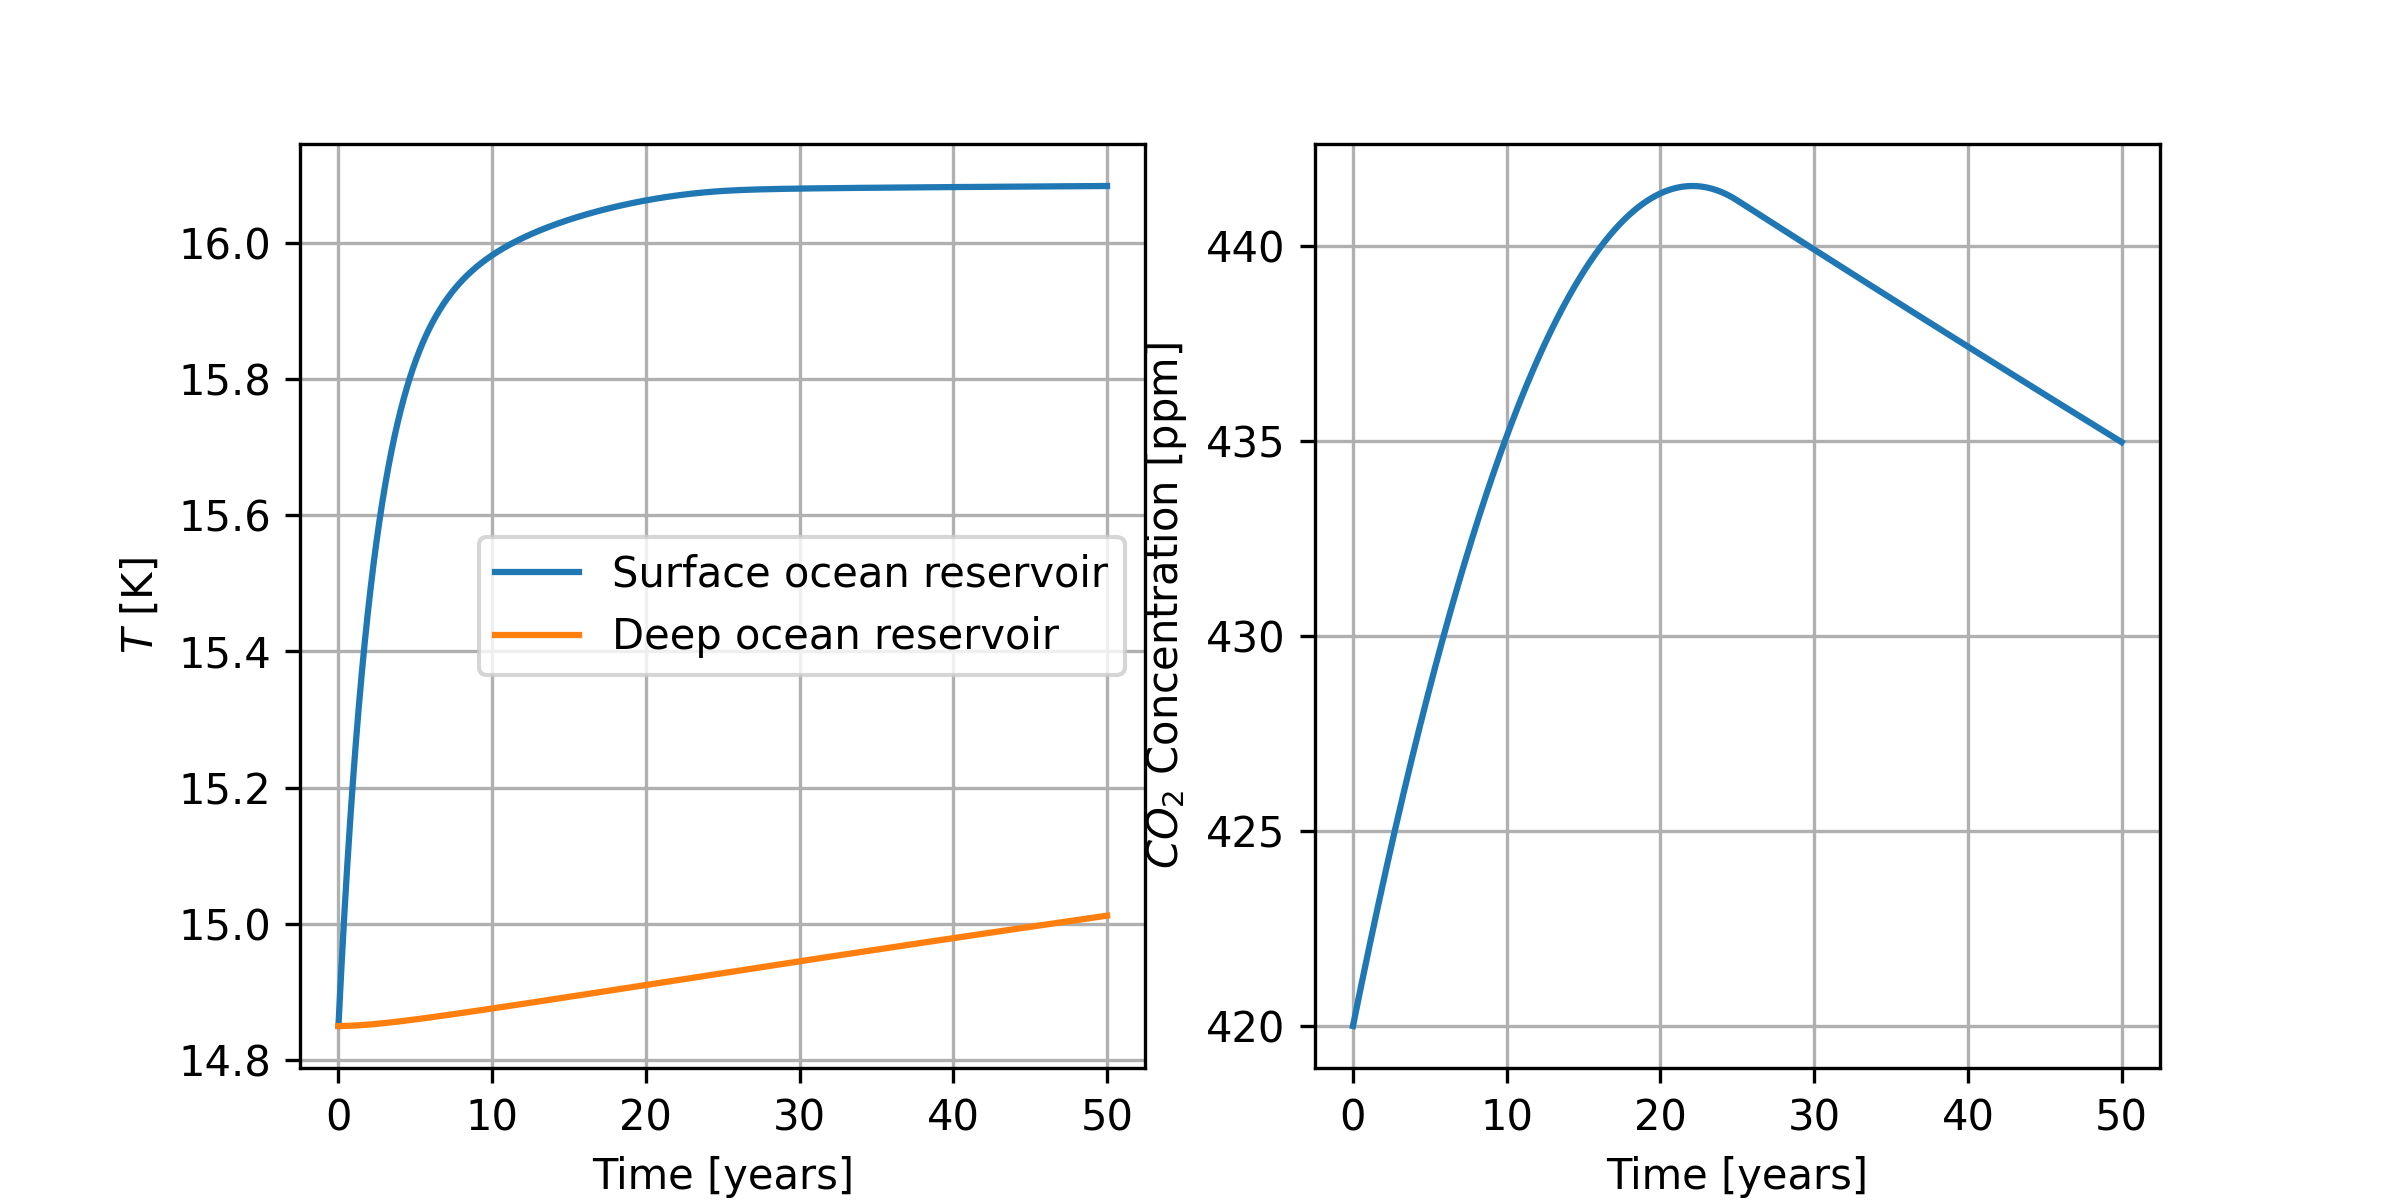
\includegraphics[width=0.8\textwidth]{figures/model.png}
    \caption{Model results for linearly decreasing emissions to net zero by 2050}
\end{figure}


\begin{figure}[H]
    \centering
    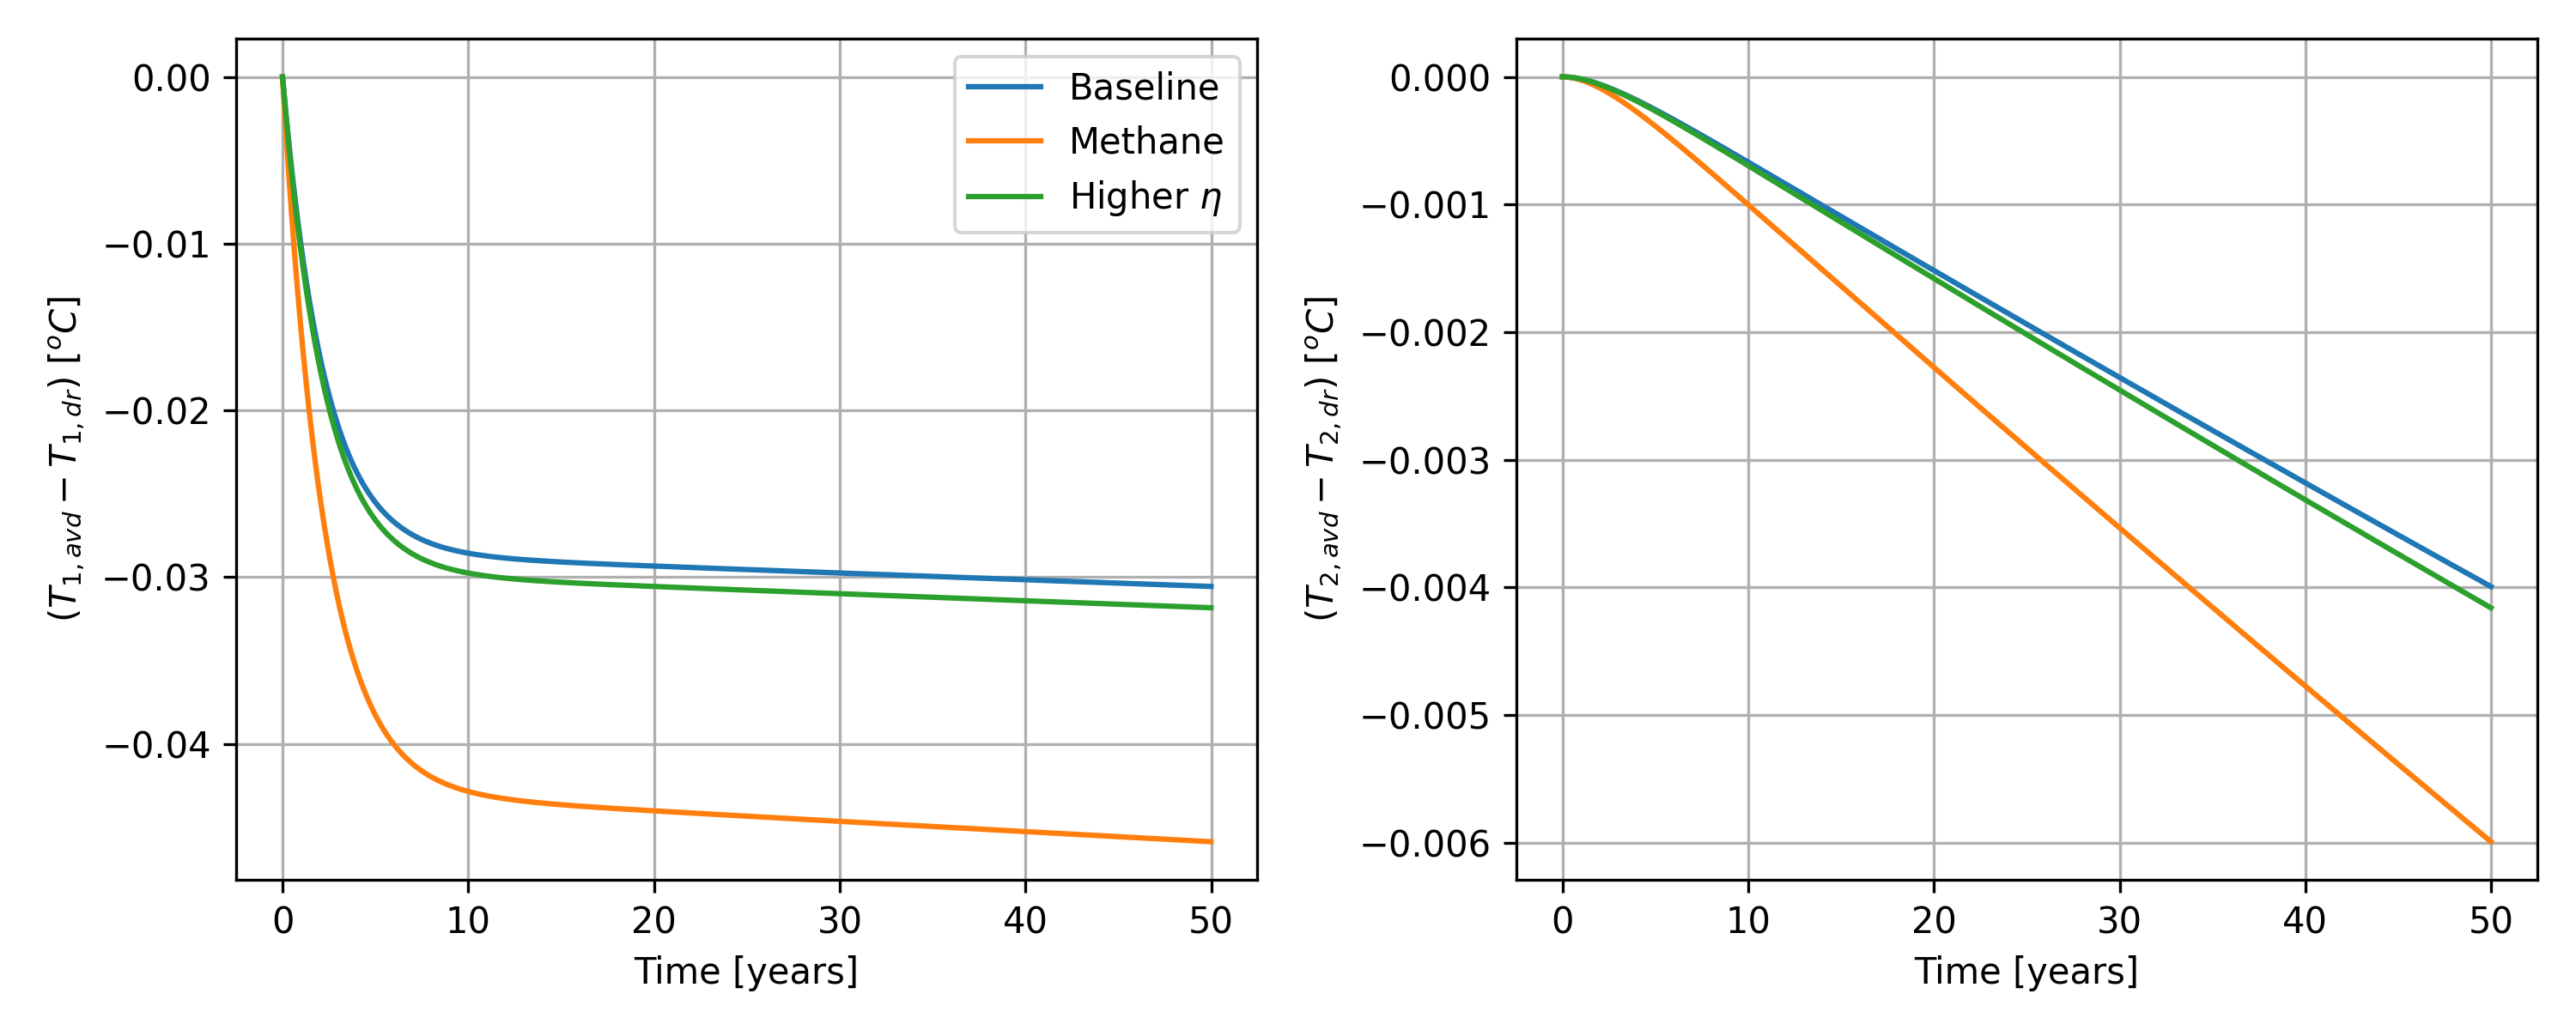
\includegraphics[width=0.9\textwidth]{figures/avoidance_comparison.png}
    \caption{Impact of global contrail avoidance for the various cases}
\end{figure}


\section{Discussion}
% discussion of results whatever they look like

\section{Conclusion}

\section{Appendix}

\begin{figure}[H]
    \centering
    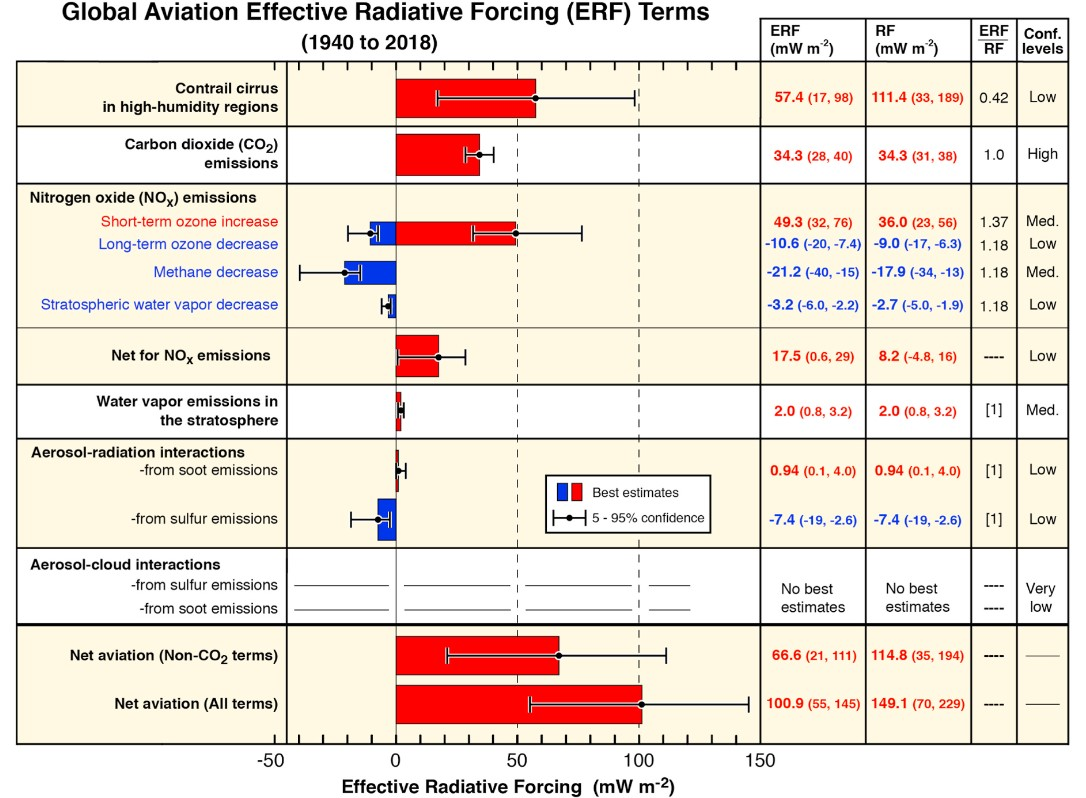
\includegraphics[width=0.7\textwidth]{figures/DSLee_ERFtable.jpg}
    \caption{Table of effective radiative forcing (ERF) in $mW/m^2$ by D.S.Lee et al. \cite{contrail_radiative_forcing}}
    \label{fig:rf_table}
\end{figure}

\begin{thebibliography}{9}


    \bibitem{co2_modelling}
    R. H. Socolow and S. H. Lam
    \emph{Good enough tools for global warming policy making}
    Department of Mechanical and Aerospace Engineering, Princeton University,
    Princeton, NJ 08544, USA

    \bibitem{rf_greenhouse}
    G. Myhre et al.
    \emph{New estimates of radiative forcing due to well mixed greenhouse gases}
    Geophysical Research Letters, Vol. 25, No. 14, 1998

    \bibitem{contrail_radiative_forcing}
    D. S. Lee et al.
    \emph{The contribution of global aviation to anthropogenic climate forcing for 2000 to 2018}
    Atmospheric Environment, 2020

    \bibitem{lagentrainment}
    Green J E, Weeks D J and Brooman J W F,
    \emph{Prediction of turbulent boundary-layers and wakes in compressible flow by a lag-entrainment method.}
    ARC

    \bibitem{esdu}
    ESDU 99032
    \emph{VGK Method for Two-Dimensional Aerofoil Sections. Part 5. Design to Specified Upper Surface Distribution}
  
\end{thebibliography}

\end{document}